%!TEX root = ../thesis.tex

\chapter{Infrastructure}
\label{sec:infrastructure}

The infrastructure implements a server-client design pattern and is divided into two parts:
The \emph{Server} part and the \emph{Local} part.
First, the server is an independent unit providing a public API to its clients.
Second, the local part is a client consuming the provided API to retrieve configuration from the server and populate it with data gathered from the deployed residential infrastructure.
Both parts will be explained in the following sections.

\section{Server Infrastructure}
\label{sec:server_infrastructure}

The server is the main storage and communication center of this project.
It persists data collected by the local deployment as also organizational information and heating schedules provided by the user via the Mobile App.

\subsection{Design Goals}

\begin{itemize}
\item \emph{Modularity} for independent, interchangeable components for improved Maintainability.
\item \emph{Extensibility} to easily add new resources and relationships.
\item \emph{Usability} for developers.
\item \emph{Testability} for good and comprehensible tests.
\end{itemize}

\subsection{Platform and Frameworks}

The server is implemented with Python, a general-purpose, multi-paradigm programming language\footnote{\url{https://www.python.org/}}.
Python was chosen as it is suitable for developing a solid web server as also for usage on restricted hardware like the Raspberry Pi used for the local deployment.
Django is a popular, open-source web application framework\footnote{\url{https://www.djangoproject.com/}} based on a model-view-controller (MVC) pattern facilitating the development of complex, database-driven web applications.
The Django REST Framework\footnote{\url{http://www.django-rest-framework.org/}} extends Django to support the design of RESTful Web APIs.

\subsection{RESTful API}

The server provides a RESTful\footnote{Note: REST is a programming paradigm where as RESTful is used to describe a web application implementing such an paradigm.} API to access a persistent storage providing the basic CRUD operations: Create, Read, Update and Delete.
Representational State Transfer (REST) is a programming paradigm used in distributed systems especially for machine-to-machine communication.
RESTful web services use HTTP as their preferred communication protocol.

REST is about resources.
Each resource is identified by a uniform resource identifier (URI) and is accessible via the request methods defined in HTTP.
There are two major types of URIs, resource collections and resource representations.
First, a resource representation is a view of its resource's state and is encoded in a transferable format.
This project uses the simple JavaScript Object Notation (JSON) format to represent resources.
Second, resource collections contain representations of the same type of a resource.

\paragraph{Design Decisions}

\begin{enumerate}
    \itemsep0em
    \item The underlying model hierarchy is represented via nested URLs.
    \label{enum:design_decision_nested_urls}
    \item The resource identifier is the first field in each resource representation.
    \item Within resource representations, collections are referenced per URL. Resources are referenced by including their representation.
    \label{enum:design_decision_resource_referencing}
    \item URL fields are identified by the name \emph{url} or the suffix \emph{\_url}. Each resource representation contains its own URL in the field \emph{url}.
    \label{enum:design_decision_url_fields_prefix}
\end{enumerate}

See Listing~\ref{lst:room-json-example} for an example of a resource representation.

\begin{snippet}[language=JavaScript,label={lst:room-json-example},caption={Example representation of the Room resource at \nolinkurl{http://server/residence/04891BB9232584/room/2/}. The \emph{url} field determines the URL of the represented resource. Within the \emph{residence} field the representation of the associated Residence resource is nested. The included Residence representation has its own \emph{url} field. Collections of the Residence's Rooms and Users are not nested but referenced via URL to limit the response size.}]
	{
		"id": 2,
		"url": "http://server/residence/04891BB9232584/room/2/",
		"name": "Dining Room",
		"residence": {
			"rfid": "04891BB9232584",
			"url": "http://server/residence/04891BB9232584/",
			"rooms_url": "http://server/residence/04891BB9232584/room/",
			"users_url": "http://server/residence/04891BB9232584/user/"
		},
		"thermostats_url": "http://server/residence/04891BB9232584/room/2/thermostat/"
	}
\end{snippet}


\paragraph{Browsable API}

The Django REST Framework offers the ability to dynamically generate a browsable interface accessible per web browser.
It includes a formatted output of the JSON response, offers forms to add new resources and edit or delete existing resources and displays URLs as clickable hyperlinks.
This interface is an additional HTML output format enabling developers to easily interact with the API without the need of external tools.
The Browsable Web API is designed for readability where as the API renders its data as compressed JSON to reduce transmission bandwidth.
See Figure~\ref{fig:server_infrastructure_browsable_api} for an example.

\begin{figure}[h]
	\begin{center}
		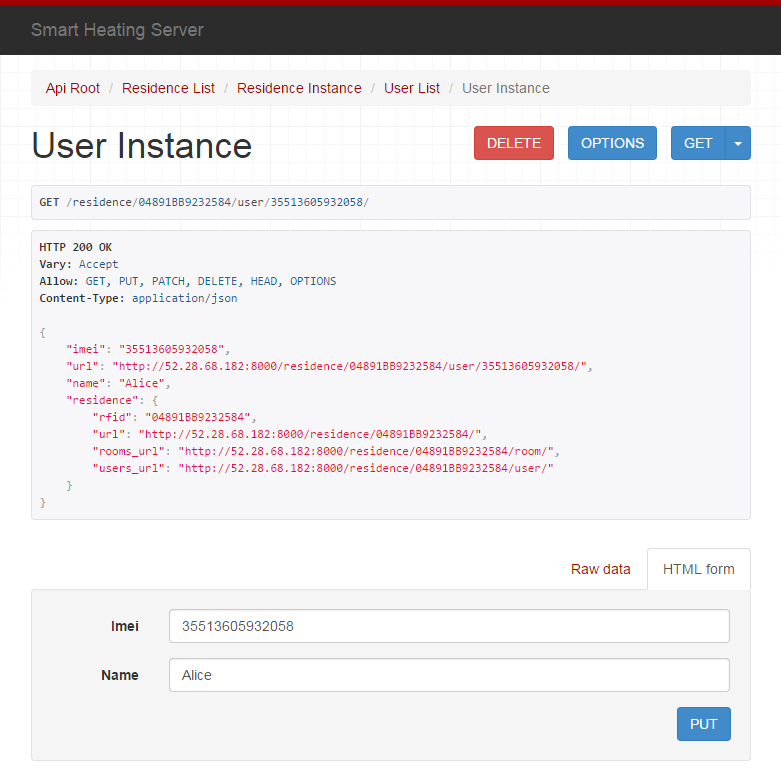
\includegraphics[width=0.8\textwidth]{images/server_browable_api_user_instance.png}
	\end{center}
	\caption{Screenshot of the Browsable Web API showing an instance of an user resource. The interface allows the developer to easily edit or delete the user as well as to navigate the residence or its associated room or user collection.}
	\label{fig:server_infrastructure_browsable_api}
\end{figure}


\subsection{Program Architecture and Implementation}

The server implementation is built on the Django Framework following a variation
%\footnote{For the interested reader: \url{https://docs.djangoproject.com/en/1.8/faq/general/\#django-appears-to-be-a-mvc-framework-but-you-call-the-controller-the-view-and-the-view-the-template-how-come-you-don-t-use-the-standard-names}}
of the Model-View-Controller (MVC) architectural pattern\footnote{\url{https://en.wikipedia.org/wiki/Model-view-controller}}.
We assume the user to be familiar with the common MVC pattern.
\todo{Explain Djangos architecture?}

\subsubsection{Models}
\label{sec:server_infrastructure_models}

Models structure the underlying data and provide operations for manipulating it.
In Django models contain the business logic and are also responsible for validating user input and providing appropriate error messages.
The \emph{smart\_heating.models} namespace contains all project models.
Each model extends the abstract \emph{Model} class providing a general method used to get an objects representation for debugging purposes as well as the abstract \emph{get\_recursive\_pks} method.
The later method is used to generate hierarchical URLs and will be further described in Section~\ref{sec:server_infrastructure_serializers}
% A high level description of all used models is given in Section~\ref{sec:system_overview_models}. 

\begin{figure}[h]
\begin{center}
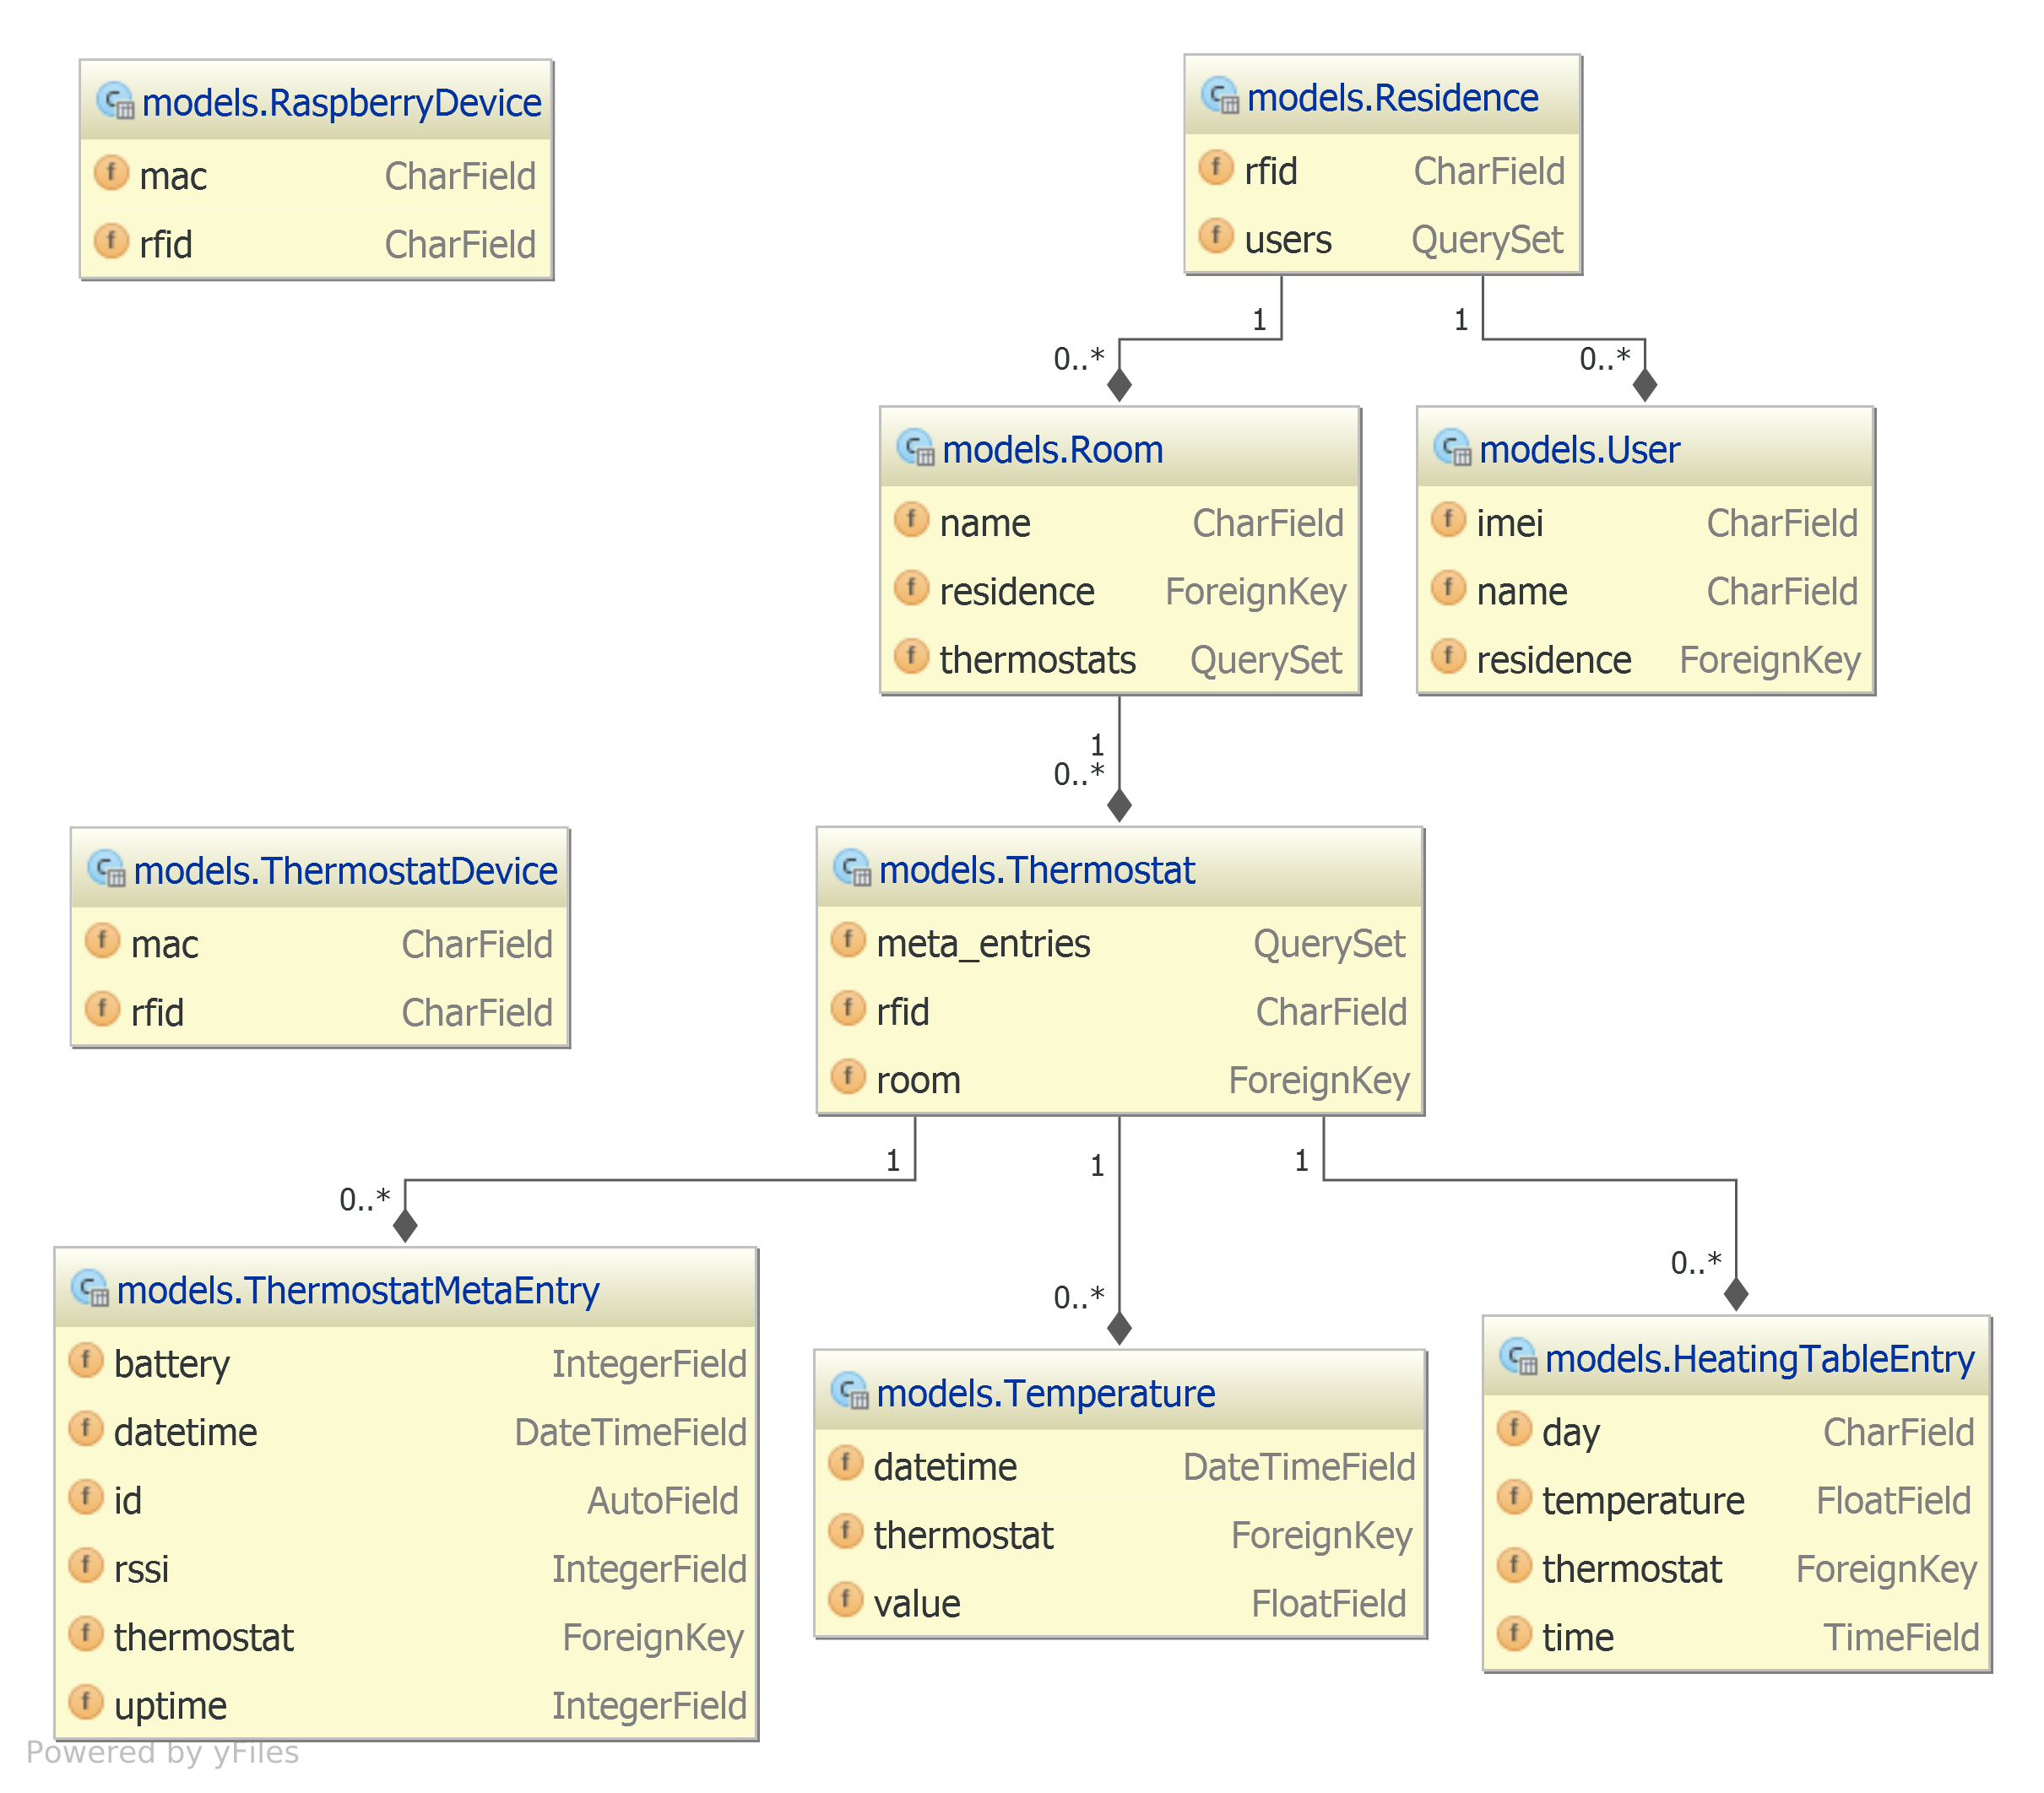
\includegraphics[width=0.8\textwidth]{images/uml_class_diagram_pycharm_highres.png}
\end{center}
\caption{UML class diagram of the models.\todo[inline]{Fix diagram: add all or remove all Querysets. Decide whether or not to display unique constraints.}}
\label{fig:class_diagram}
\end{figure}

Thermostats are organized within rooms and belong to a residence. See Figure~\ref{fig:class_diagram} for a graphical representation of the used models.

\paragraph{Residence}

is identified by the radio frequency identification (RFID) tag number on the deployed local communication gateway. A residence combines users and rooms with their associated thermostats and data into a single encapsulated unit.

\paragraph{User}

is identified by the smart phone's serial number\footnote{The International Mobile Equipment Identity (IMEI) is a 15-digit serial number associated to each GSM cell phone.} and can be registered to at most one residence.

Room, Thermostat, Temperature, Heating Table Entry, Meta Entry
\todo[inline]{Finish models}

% temperatures and other data from the local deployment as also the heating schedule from the mobile app.

\subsubsection{Serializers}
\label{sec:server_infrastructure_serializers}

Serializers are responsible for translating models into a transmittable format and reverse.
This project uses JSON as the transmittable format.
Each model has an associated serializer which determines which model fields should be included into the resource representation.
Additional fields can be added to the representation or individual field representations can be overwritten to offer customized output.

A commonly used customization is the replacement of the default \emph{HyperlinkedIdentityField} with \emph{HierarchicalHyperlinkedIdentityField}.
This custom serializer field generates URLs according to the hierarchical schema applied in this project.
For example the URL for a room would be \nolinkurl{http://server.com/residence/041FB2B9232580/room/5/}.
To assemble this URL not only the identifier of the room but also the identifier of its parent are required.
The adapted field extends the default field and provides all identifiers of the hierarchy required to generate the URL by using the hierarchical base class \emph{smart\_heating.models.Model}.

Nested resources are implemented using nested serializers.
This way existing serializers can be reused to include their resource representation into another representation.
% \item Within resource representations, collections are referenced per URL. Resources are referenced by including their representation.


\subsubsection{Views}
\label{sec:server_infrastructure_views}

A view is a class which processes requests and returns a response.
Django offers generic view classes and mixins providing common functionality and to facilitate code reuse.
The Django REST Framework further abstracts views by supplying \emph{ViewSets}.

Custom pagination for expectedly large collections as temperatures or meta entries.

\subsubsection{Routers}
\label{sec:server_infrastructure_routers}



\subsection{Automated Testing}

Automated software testing is an important part of this project. Django and also the Django REST Framework facilitate automatic testing by providing several classes and tools helping to write and execute tests. Automatic software testing allows the application of test-driven development practices to ensure high software quality.

Furthermore the usage of an Continuous Integration service like Travis CI\footnote{\url{https://travis-ci.org/}} ensures the periodic execution of all tests and logging of the test results.

\subsubsection{Tests as Documentation}

Tests as Documentation complement traditional documentation.

\todo[inline]{Listing of test output}

\section{Local Deployment}
\label{sec:local_infrastructure}

The local deployments consists of the residential communication gateway and the deployed thermostats with their wireless adapters. The communication gateway collects the data read from the thermostats and sends it to a remote web server. The thermostats are programmable and allow us to modify their behaviour by replacing and adapting the flashed firmware. This project uses the work of previous lab projects as a basis to build upon. The primary focus is to improve the basic functionality of the communication gateway and create an unified but loosely coupled infrastructure by using the RESTful API provided by the server.
See also Figure~\ref{fig:residence_layout} for an overview of the local deployment.

\begin{figure}[h]
\begin{center}
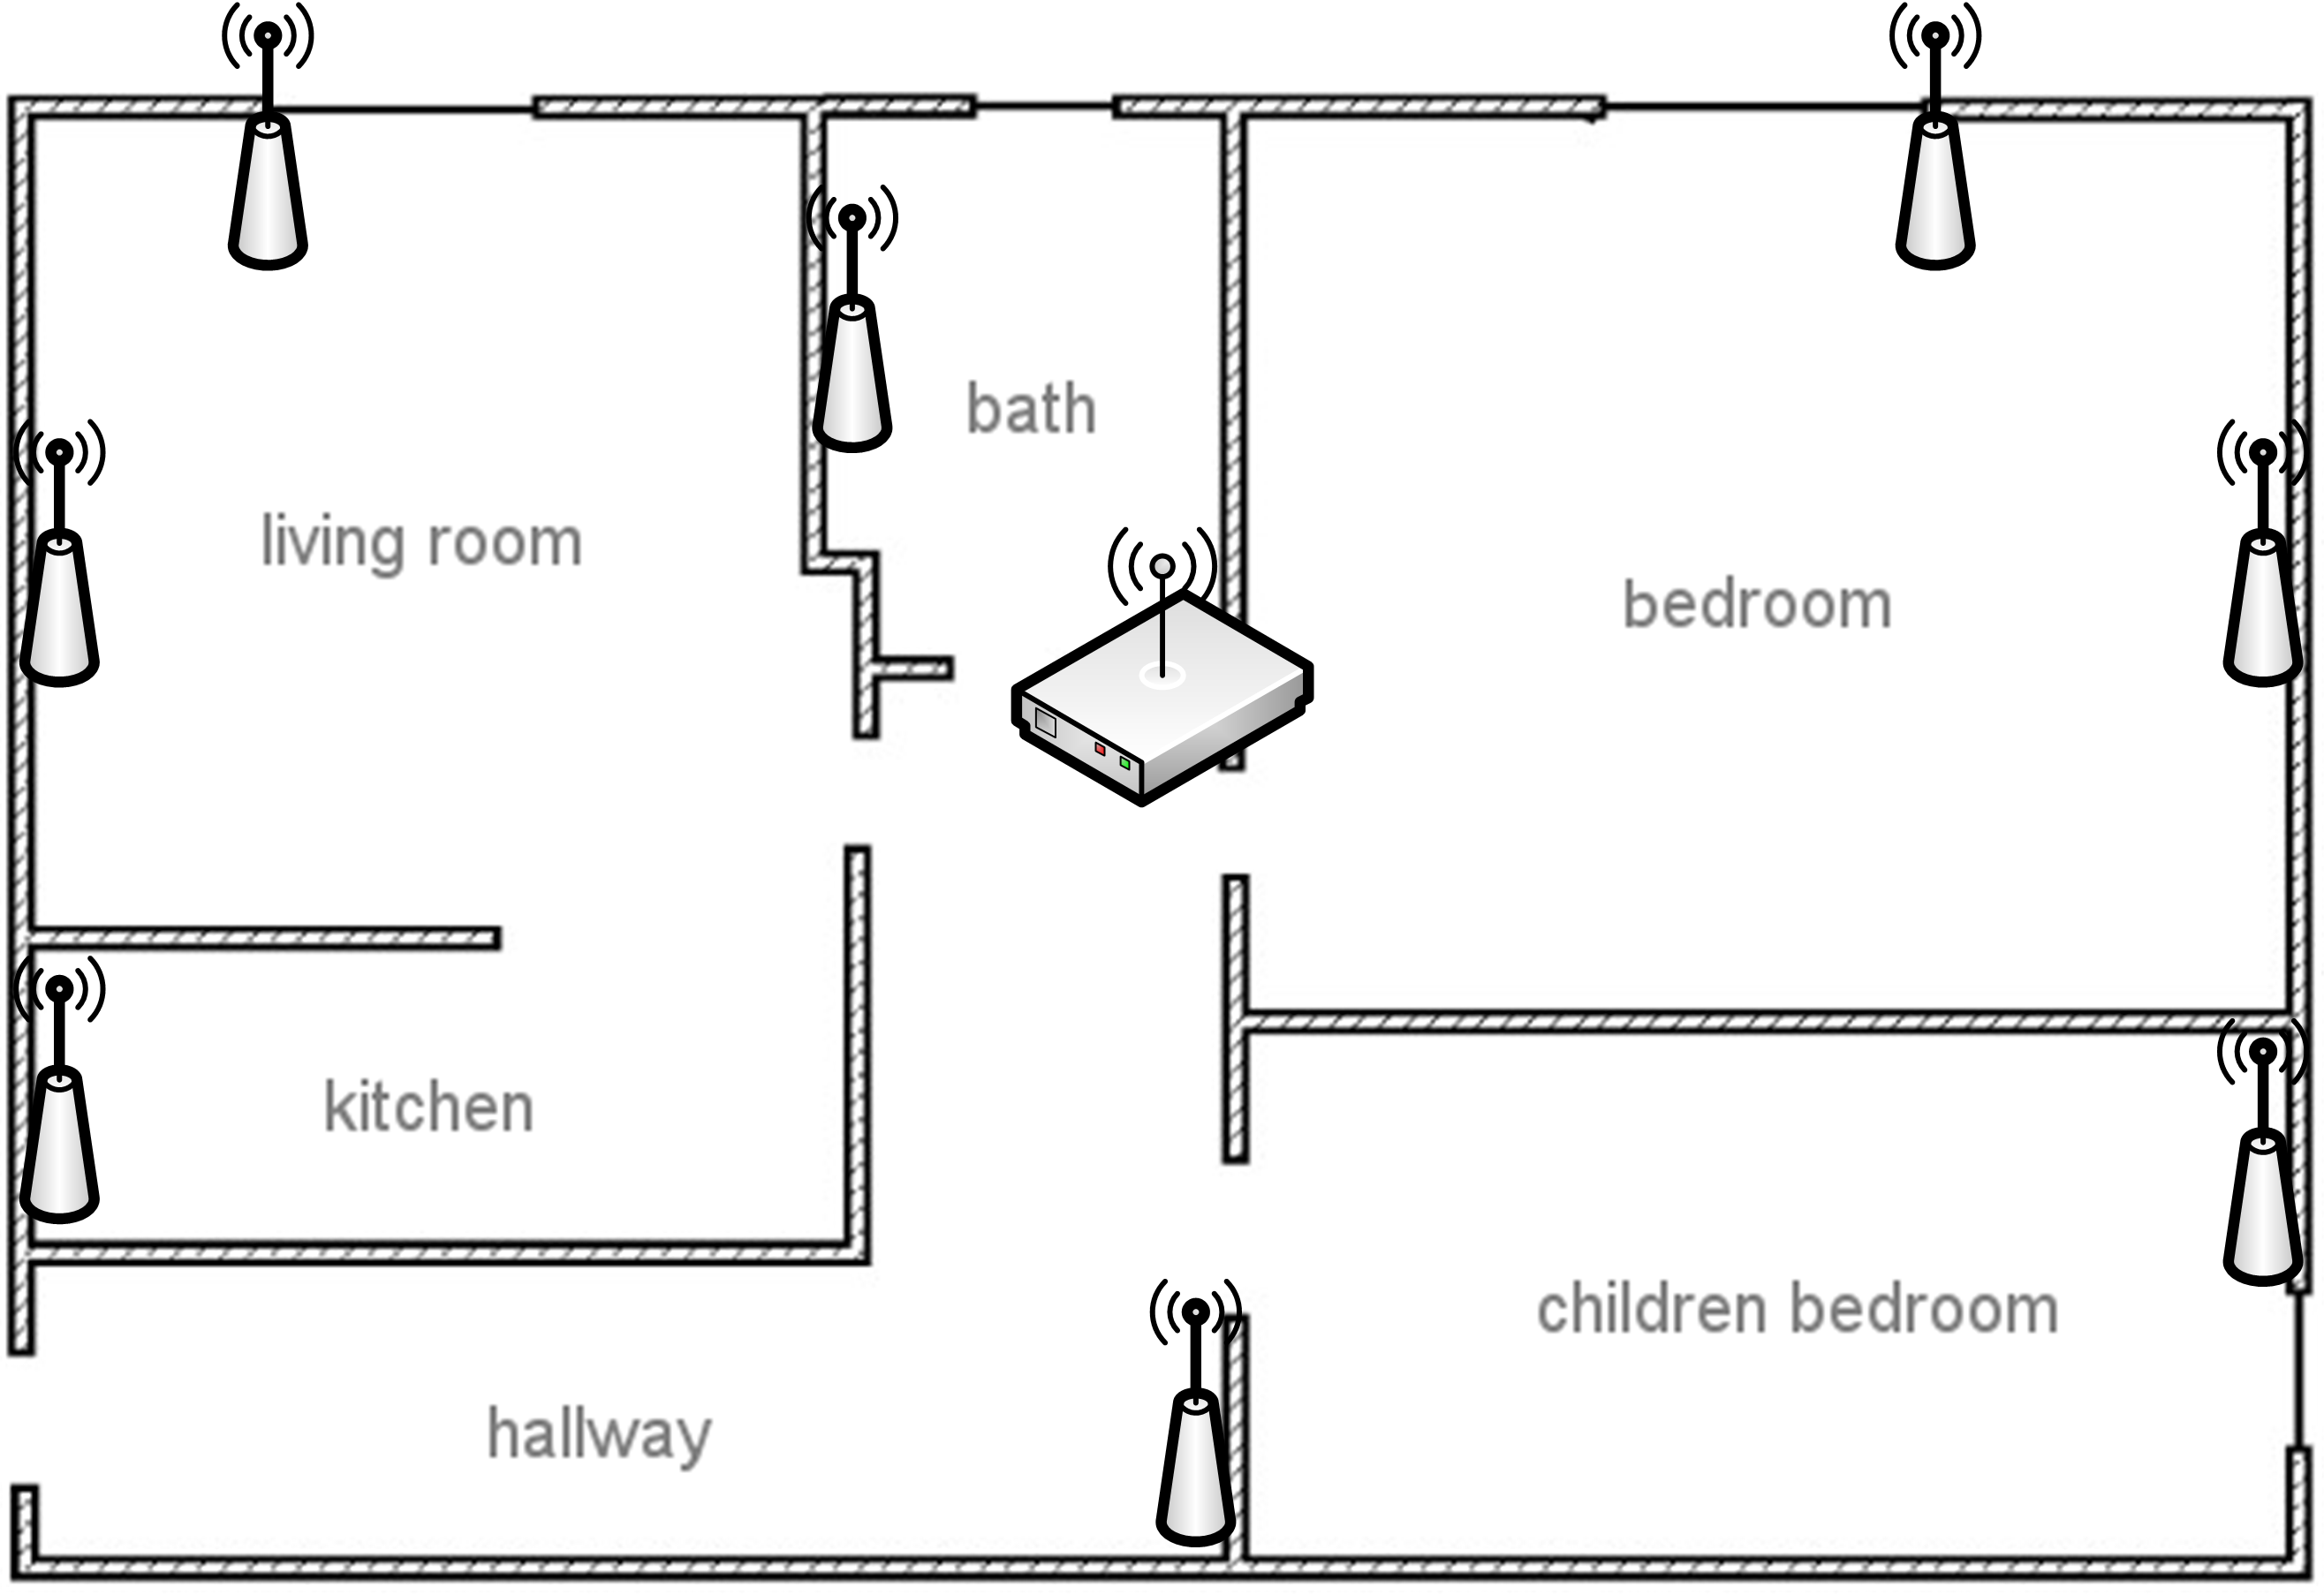
\includegraphics[width=0.8\textwidth]{images/residence_layout_schema.png}
\end{center}
\caption{Example of a residence layout depicting a possible deployment. The local communication gateway is installed in the hallway, connected to the internet and has wireless connections to the deployed thermostats represented as antennas. Source of the original image: \url{http://www.haus-topplicht.de/wp-content/uploads/2013/12/planwohnung2.jpg}}
\label{fig:residence_layout}
\end{figure}

\subsection{Existing Infrastructure}

This lab project builds upon work previously done at the Distributed System Group\footnote{\url{https://www.vs.inf.ethz.ch/}}. 

\subsubsection*{Hardware}

Thermostats, etc

\subsubsection*{Software}

Willis Scripts

\subsection{Design Goals}

Simple, Reliable, Failure resistant

\subsection{Platform and Frameworks}

tunslip6, Python, COAP, aiocoap, requests

\subsection{Implementation}

The communication gateway collects, caches and processes the data read from the thermostats as also the control commands from the server. The local communication gateway works as a proxy server and enables the local deployment to operate independently from the connection to the remote server. This way the last downloaded heating schedule is kept and operated until the server connection is be reestablished. 
%Die grundlegende Einheit jedes Deployments ist die Residence. Eine Residence entspricht genau einem installiertem lokalen System, das die gelesenen Daten der Thermostate sowie Steuerbefehle des Servers sammelt, cached and ausführt. Das lokale Gerät arbeitet als ein lokales Gateway und sorgt dafür, dass der lokale Teil unabhängig von der Verbindung mit dem remote Server funktioniert.
% Temperaturen und andere Meta-Daten von den angebundenen Thermostaten sammelt und cached.

